\begin{multicols}{2}
\subsection*{INTRO}
이번주차 실험에서는 MAC (Medium Access Control) 을 다룬다.  Data Link Layer에서 다루는 기능인 data link control에서 error detectiion 과 재전송등의 process를 관장하는데, 네트워크에서 한 회선에서 여러 디바이스가 공유하는 상황에서 어떻게 control 하는지 알아본다. 이러한 회선을 공유하는 상황에서 2개이상의 신호가 겹치면 데이터의 수신율이 떨어진다. 즉 shared link에서 한 디바이스만이 전달을 하게 하는것이 multiple access resolution이고 이때 사용하는 protocol을 MAC 이라고 한다. 그중접속하는 각 디바이스의 전달시간을 random 시간에 의존하여 collison을 회피하는 protocol을 Random Access Protocols 라고한다. 이중 ALOHA, CSMA, CSMA/CA에 대해서 다루도록 한다.
%
%               Section 1 
%
\vspace{-4mm}
\section{ALOHA}
\vspace{-2mm}
\subsection{PURE ALOHA}
가장 기본적인 random access protocols이다. Shared Network 에서 어떤 device가 전송을 random 시간에 의존해서 ACK 신호를 보내고, 이를 수신받지 못하는 상황을 collison이 발생한다고 인지한다. 그럼 해당 네트워크에 접속한 이후  collison 횟수를 count 하고, count 수를 $k$라고 할때 0 부터 $2^{k-1}$의 대기시간을 가지며 재전송을 진행한다.  이렇게 BEB\footnote{binary exponential backoff}로 재전송시간 term을 정해주면 언젠가는 collison이 일어나지 않을것이다. \\
    \begin{minipage}{\columnwidth}
    \vspace{2mm}
    \centering%
    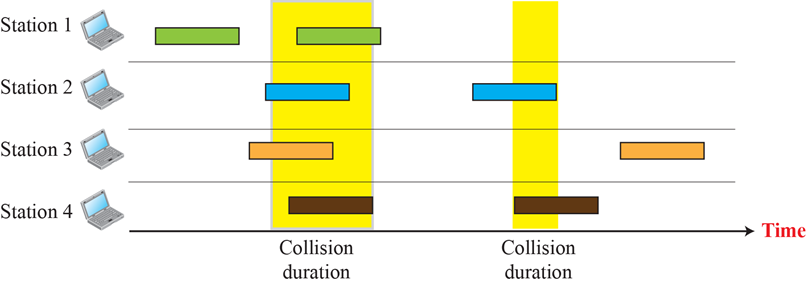
\includegraphics[width=.9\columnwidth]{image/week12/1-1.png}
    \captionof{figure}{\small Pure Aloha Diagram}
    \vspace{-4mm}
    \end{minipage}
\vspace{-2mm}
\subsection{SLOTTED ALOHA}
Slotted Aloha는 Pure Aloha의 높은 Collison 발생가능성을 개선하기 위해 고안된 protocols이다. Slot이란말 그대로 Pure Aloha에서 전송가능한 시간의 space가 연속적이었다면 , 이를 일정한 timestep을 가지는 step으로 제한하여 각 slot 시간 사이에서 전송을 하고자 하는 device의 frame 전송시간을 각각 slot 사이로 특정함으로서 collison 확률의 발생을 줄인 protocols이다.
    \begin{minipage}{\columnwidth}
    \vspace{2mm}
    \centering%
    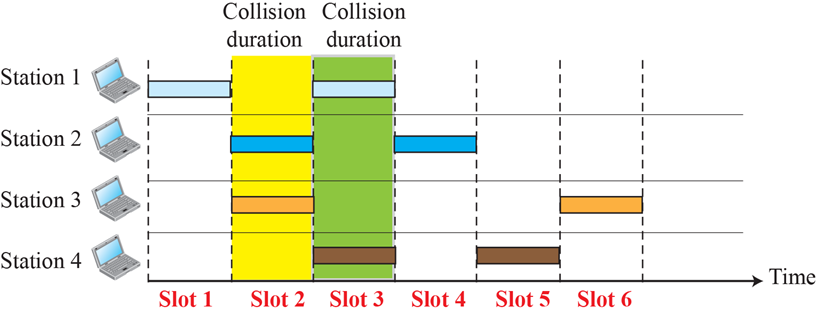
\includegraphics[width=.9\textwidth]{image/week12/1-2.png}
    \captionof{figure}{\small Slotted Aloha Diagram}
    \vspace{-4mm}
    \end{minipage}
\vspace{-2mm}
\subsection{Comparison of throughput between pure-aloha and slotted-aloha}
Throughpput은 단위시간동안 보내는 packet의 개수로, 성공적인 Frame 전송의 평균값을 의미한다.
\vspace{-4mm}
\subsubsection*{Vulnerable Time : Pure Aloha}
\vspace{-2mm}
shared link에서 한 device가 전송중에 있으면 다른 device또한 이시간동안은 다른 device에서도 전송을 하면 collision이 발생하게 된다. Vulnerable time은 한 device가 어느 구간에서 어느 구간까지 전송이 없어야 성공적으로 frame을 보낼 수 있는지 판단하는 최소의 단위다.
이때 문제를 단순화하고 2 aloha protocol을 비교하기 위해서 단위를 통일시켜보자. 각 frame이 전송되는 시간을 $T_{fr}$  이고 모든 device에서 동일하다고 할때, Pure Aloha에서는  figure와 같이 전송시간이 정해지지 않았기때문에 collison 이 발생할 수 있는 time domain은 2개의 frame의 전송시간의 합인 $2T_{fr}$이 vulnerable time이 된다.\\
    \begin{minipage}{\columnwidth}
    \vspace{2mm}
    \centering%
    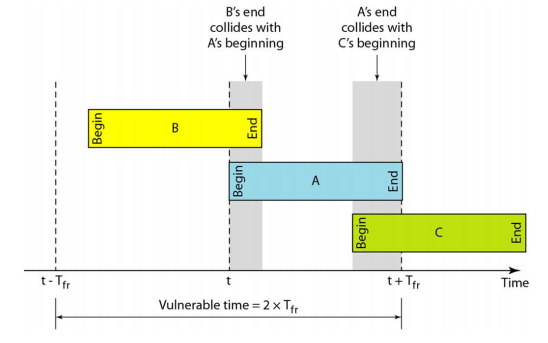
\includegraphics[width=.9\textwidth]{image/week12/1-3.png}
    \captionof{figure}{\small Concept of Vulnerable time}
    \vspace{-4mm}
    \end{minipage}
\vspace{-2mm}
\subsubsection*{Vulnerable Time : Slotted Aloha}
\vspace{-2mm}
반면 slotted aloha에서는 각 frame의 전송시간이 $T_{fr}$로 통일될때, 최적의 slot 길이는 $T_{fr}$ 이므로 slotted aloha 의 vulnerable time은 $T_{fr}$ 이다.\\
\end{multicols}
\clearpage 
\begin{multicols}{2}
\vspace{-2mm}
\subsubsection*{Throughput}
\vspace{-2mm}
Throughput은 아래의 equation과 같이 표현할 수 있다. 이때 $G-\text{load}$ 는 주어진시간동안 전송을 시도한 평균횟수이다. 
$$
S(\text{throughput}) = P_{success} \times G-\text{load}
$$
일정시간동안 발생하는 횟수에 관한 문제이므로, frame을 한 device에서 전송하는 과정을 poison process로 모델링 할 수 있다.이때 전송을 시도하는 확률을 $\lambda$ 라고할때,   T 시간동안 K번 frame이 도착하는 $P_{success}$ 는 $P[\text{k arrivals in T seconds}] = \frac{(\lambda T)^k}{k!} e^{-\lambda T}$로 표현할 수 있다.  $\lambda$ 는 앞서 정의해준 G-load에서 성공할 수 있는 최소의 단위시간인 vulnerable time 으로 나눈값으로  표현할 수 있으므로 :
\begin{align*}
  P_{\text{sucess}} &= p[\text{G-load in vulnerable time}]\\
   &= p[\text{k  transimssions in vulenrable time}] \\
   &= \frac{(\lambda T)^k}{k!} e^{-\lambda T}
\end{align*}
이때 pure aloha의 vulnerable time 은 $T_{fr}$, slotted aloha는 $2T_{fr}$ 이고 $\lambda = G / \text{vulnerable time}$ 이므로 : 
$$
S(\text{throughput})= P_{\text{success}} \times G =
\begin{cases}
\frac{(2G)^k}{k!}e^{-2G}, & \mbox{pure aloha case}\\
\frac{(G)^k}{k!}e^{-G}, & \mbox{slotted aloha case}
\end{cases}
$$
각각의 G에 대한 throughput graph를 확인하면, 각 G-load 가 1/2 , 1일때 slotted aloha가 pure aloha보다 2배의 throughput을 frame의 을 slot과 slot 사이에서만 가능하게 함으로서,  개선한 부분을 확인할 수 있다\\
    \begin{minipage}{\columnwidth}
    \vspace{2mm}
    \centering%
    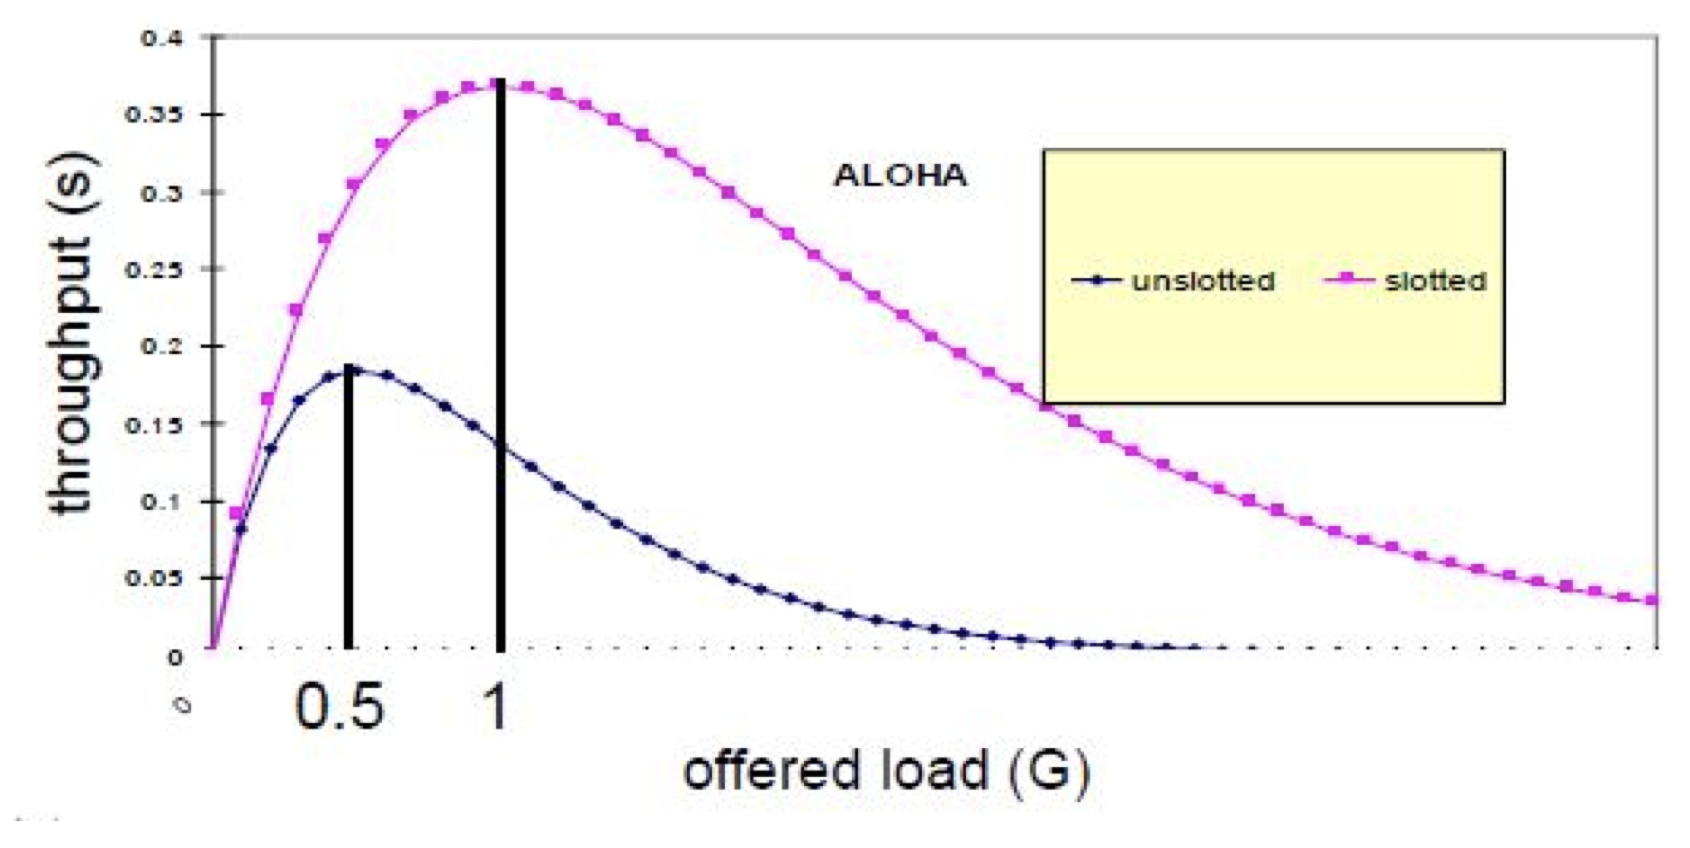
\includegraphics[width=.9\textwidth]{image/week12/1-4.png}
    \vspace{-2mm}
    \captionof{figure}{\small Aloha's throughput graph }
    \vspace{-4mm}
    \end{minipage}
\vspace{-2mm}
%
%               Section 2
%
\section{CSMA}
앞서 aloha에서는 전송을 시작하고 ACK이 돌아오는 여부로 collision을 판단하는 프로토콜을 이용했지만, 전송을 시도하기 전 매체에서 전송이 있는지 탐지하면 collision의 발생을 줄일 수 있다. CSMA 에서 ‘Carrier Sensing’의 주된 게념은   전송전 listen의 동작을 통해서 채널이 사용중 (busy)인지, 아닌지 (idel) 반송파 검출(carrier sense)\footnote{carrier sense는 각 노드가 자신의 신호를 반송파 매체 (Carrier)에 실려보내기 전에 먼저 선점되었는지를, "Listen before Talk"를 요구하는 의미에서 사용된 terminology 이다.}를 통해서 판단하고 , 채널이 idle 이면 전송을 시작하는데 이때 idle를 인지하고 직후 어떤 행동을 하는지에 따라 작동방법을 분류할 수 있다.\\

즉, CSMA의 carrier sensing 에 대한 작동방법은 전송하고자 하는 channel이 busy일때 node가 어떻게 동작하는지에 대한 지속방식(pessistance mechanism)에따라 나뉜다.  예를들어 한 디바이스에서 채널이 idle하다고 감지하더라도, 실제로는 다른 디바이스에서 전송한 첫번째 frame의 비트가 도달중이라 idle로 측정되는 경우와 같이 모든 collision을 방지할 수는 없다. 즉 이순간에 어떤 동작을 취할지에 따라 프로토콜이 아래 3가지로 분류 가능하다.\\
    \begin{minipage}{\columnwidth}
    \vspace{2mm}
    \centering%
    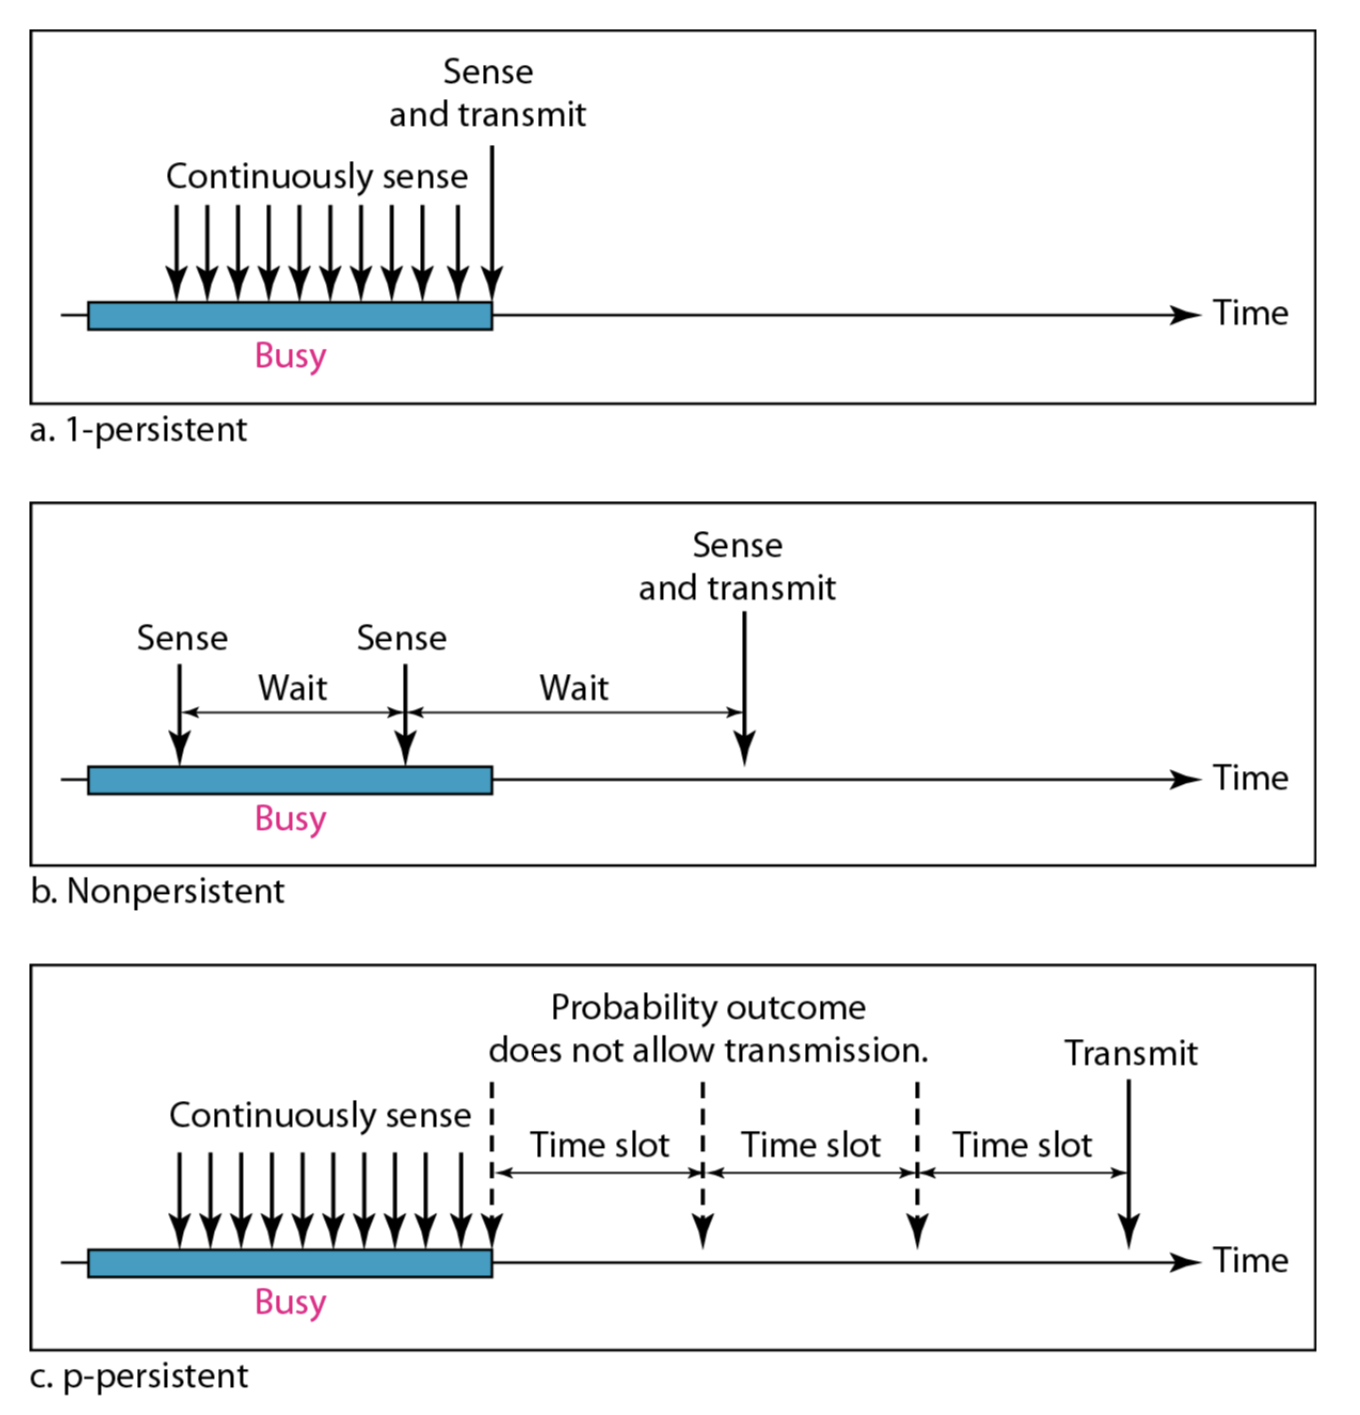
\includegraphics[width=.9\textwidth]{image/week12/2-1.png}
    \vspace{-3mm}
    \captionof{figure}{\small three types of persistance mechanism of CSMA}
    \vspace{-4mm}
    \end{minipage}
\vspace{-2mm}
\vspace{-2mm}
\subsubsection*{1-persistent}
\vspace{-2mm}
\begin{itemize}
    \item 충돌되지 않으리라는확률 1 을 갖고 사용중이지 않은 것을 감지하자마자 즉시매체에 접근하여 프레임 송출\vspace{-2mm}
    \item 충돌발생 가능성이 가장 크므로채널사용율이 낮은 대신에대기시간은 짧음\vspace{-2mm}
    \item 유선LAN이더넷에서는 바로 이렇게 행동\vspace{-2mm}
\end{itemize}
\vspace{-2mm}
\subsubsection*{nonpersistent}
\vspace{-2mm}
\begin{itemize}
    \item 반드시충돌될 것이라고 비관하여 비록 사용중이지 않은 것을 감지하여도, 확률분포에서 얻어진 임의시간 만큼 무조건 기다린 후매체접근\vspace{-2mm}
    \item 충돌이 적어채널사용율은 좋아지나,대기시간이 길어짐\vspace{-2mm}
\end{itemize}
\vspace{-2mm}
\subsubsection*{p-persistent}
\vspace{-2mm}
\begin{itemize}
    \item 사용중이지 않은 것을 감지하면,\vspace{-2mm}
    \vspace{-2mm}
        \begin{itemize}
        \item 전체중확률 p 가충돌되지 않을 것으로 판단하여매체에 접근하고\vspace{-2mm}
        \item 의심을 갖는 나머지확률 q(=1-p)는 한단위시간 만큼 기다린 후매체에  접근\vspace{-2mm}
        \end{itemize}
        \vspace{-2mm}
    \item nonpersistent 처럼충돌을 줄이고, 1-Persistent 처럼대기시간을 줄이고자 하는위 두 가지에 대한 타협안임\vspace{-2mm}
\end{itemize}

\end{multicols}
\clearpage
\begin{multicols}{2}
%
%               Section 3
%
\section{Hidden Terminal Problem}
\vspace{-2mm}
무선 네트워킹 환경에서 figure와 같이 어떤 Node가 AP(access point)에 표시되고 해당 AP와 통신하는 다른 Node에서는 표시되지 않는 문제를 의미한다.\\
    \begin{minipage}{\columnwidth}
    \vspace{2mm}
    \centering%
    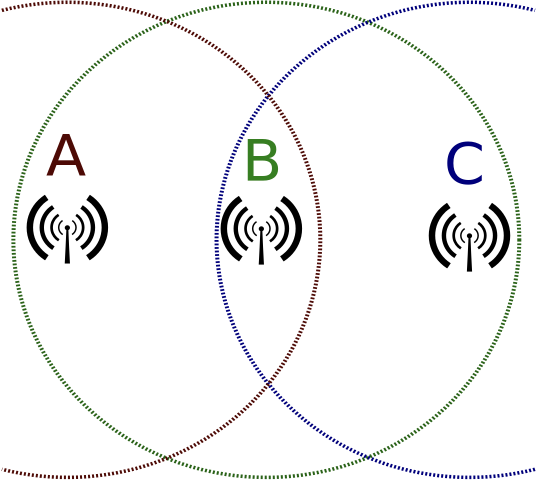
\includegraphics[width=.5\textwidth]{image/week12/3-1.png}
    \vspace{-2mm}
    \captionof{figure}{\small Hidden Node Problem Diagram}
    \end{minipage}

Node A 와 Node C는 거리가 멀어 서로의 신호를 주고 받을 수 없다. 하지만 B와 A, C는 각각 가능하다. 만약  C 에서 송신이일어날대 A에서는 신호 에너지 레벨이 낮아 Energy Detection Mechanism이 동작하지 않아 A에서 보내는 신호의 존재를 인지하지 못하고 A와 B사이에서 통신이 진행되는 유무와 관계없이, B 와 C사이의 통신이 가능하다고 판단해버린다. 이때문에  B에서 A 와 C에서 서로 인지를 못해 송신이 겹칠때 collision이 발생하게 되고 이러한 문제를 “Hidden Node Provblem”, 혹은 “Hidden Terminal Problem”이라고 한다. 

Hidden Node Problem은 4-way hand shake 방식인 RTS/CTS mechanism을 이용하여 해결할 수 있다.
\columnbreak
%
%               Section 4
%
\section{CSMA/CA Collison Avoidance : 4-WH}
\vspace{-4mm}
hidden terminal 문제를 해결하기 위해서 전송이전에 채널을 예약하는 4-Way Handshake (4-WH)CSMA/CA protocols를 이용한다.
4-WH protocols는 데이터 packet 전송 이전에 송신 터미널은 RTS(Requset To Send) Packet으로 전송하고, 수신 터미널은 이에대한 응답으로 CTS (Clear To Send) Packet을 송신 터미널에 전송한다. 이렇게 예약을 확인한 이후 송신 터미널의 데이터 packet 전송이 시작된다.\\
    \begin{minipage}{\columnwidth}
    \vspace{2mm}
    \centering%
    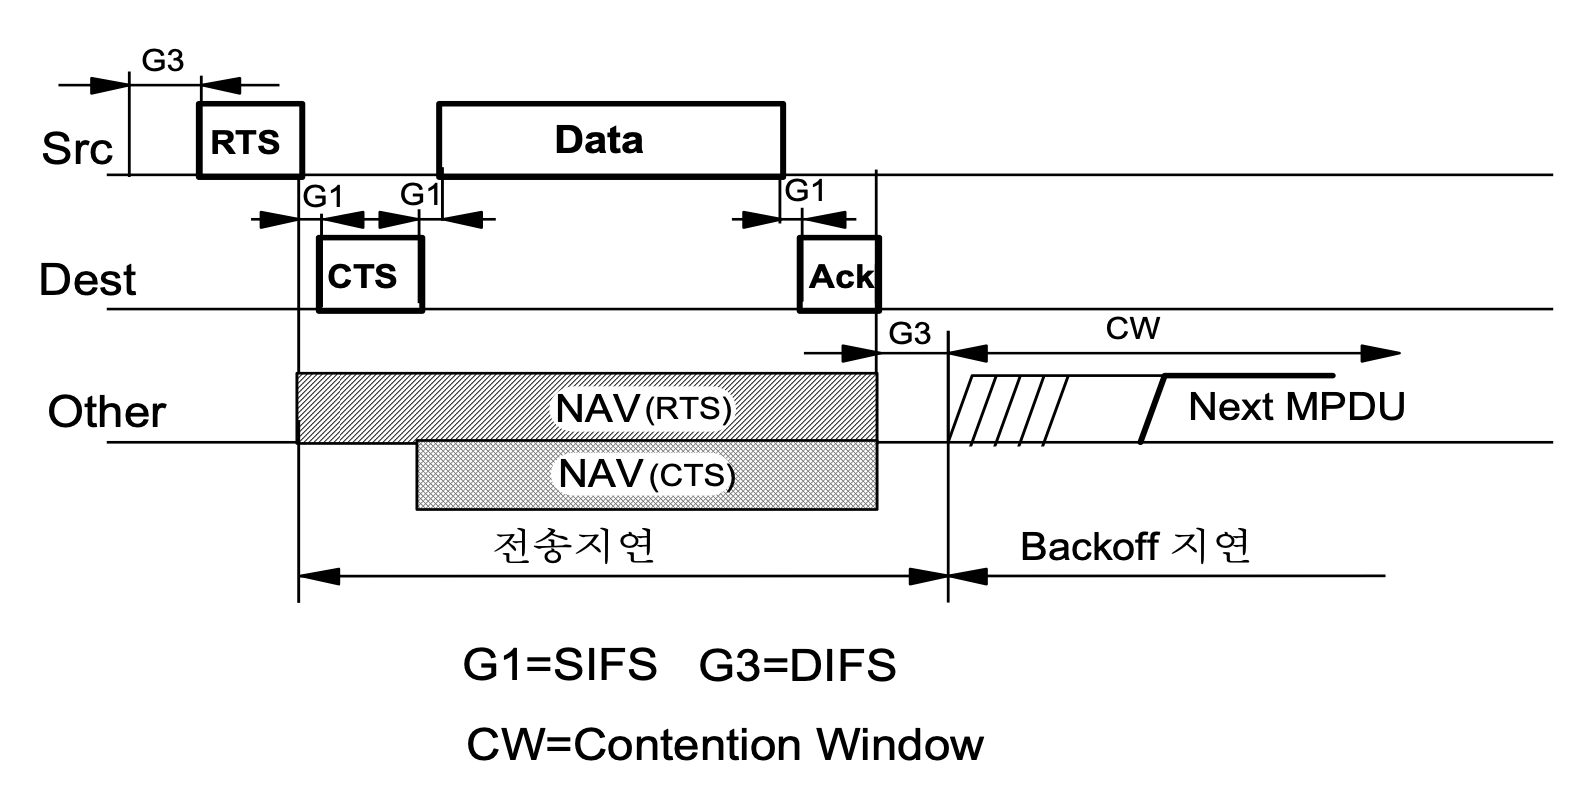
\includegraphics[width=.96\textwidth]{image/week12/4-1.png}
    \vspace{-4mm}
    \captionof{figure}{\small 4-WH CSMA/CA protocols의 packet전송 과정}
    \end{minipage}
    
% \vspace{2mm}
이때 송신 터미널에서 보내는 RTS packet와 이를 받고 송신터미널에서는 CTS packet들에는 NAV(Network Allocation Vector)정보가 포함되는데, 수신 터미널을 제외한 모든 스테이션에서는 각각 자신의 NAV를 세트하여 그 동안의 전송을 지연함으로서 RTS와 CTS 신호를 송신거리에 있는 터미널들에게서 확산시키고, 이동안 송신과 수신을 하는 터미널을 제외한 다른 터미널들은 전송을 지연함으로서 collison을 방지한다.
\end{multicols}